% ============================================================
% Compiler-as-Reward: Process Feedback for Coding Agent RL Training
% ICML 2026 Workshop: Deep Learning for Code: Human-Centered Coding Agents
% ============================================================
\documentclass[10pt]{article}

% Layout — 4-page workshop paper
\usepackage[margin=1in,top=1.1in,bottom=1.1in]{geometry}
\usepackage{amsmath,amssymb,amsthm}
\usepackage{graphicx}
\usepackage{booktabs}
\usepackage{xcolor}
\usepackage{microtype}
\usepackage{enumitem}
\usepackage{hyperref}
\usepackage{parskip}
\usepackage{titlesec}
\usepackage{caption}
\usepackage{subcaption}
\usepackage{multirow}
\usepackage{array}
\usepackage{tabularx}
\usepackage{bm}
\usepackage{pgfplots}
\pgfplotsset{compat=1.18}

% Tighter section spacing for 4-page limit
\titlespacing*{\section}{0pt}{8pt plus 2pt minus 2pt}{4pt plus 1pt}
\titlespacing*{\subsection}{0pt}{6pt plus 1pt}{3pt plus 1pt}

\setlength{\parskip}{3pt}
\setlength{\parindent}{0pt}

\definecolor{darkblue}{RGB}{0,60,120}
\definecolor{darkred}{RGB}{160,0,0}
\definecolor{darkgreen}{RGB}{0,110,0}

\hypersetup{
  colorlinks=true,
  linkcolor=darkblue,
  citecolor=darkblue,
  urlcolor=darkblue
}

% Compact caption
\captionsetup{font=small,labelfont=bf,skip=4pt}

% ============================================================
\title{\textbf{Compiler-as-Reward: Process Feedback for Coding Agent RL Training}}

\author{
  Junhao Fu \\
  \small{\texttt{junhao.fu@sorcara.com}}
}

\date{}

% ============================================================
\begin{document}
\maketitle
\vspace{-10pt}

% ============================================================
\begin{abstract}
Reinforcement learning for coding agents typically relies on sparse, binary pass/fail signals,
leading to slow convergence and reward hacking in multi-step agentic settings.
We propose \textbf{Compiler-as-Reward}: instead of hand-crafted test suites, we use real
compiler and validator feedback directly as per-step process rewards.
Building on GiGPO~\cite{zeng2025gigpo} (NeurIPS 2025), we introduce
(1) \textbf{Compiler-OPD} (Ordered Process Densification), which assigns
step-level credit based on validation outcomes during rollout; and (2) \textbf{Error-Branch},
which forks rollout trajectories at validation-failure states---the points of highest policy
uncertainty---concentrating exploration where the agent needs it most.
We fine-tune Qwen3.5-4B via GiGPO on a new 22-task Shopify Horizon theme-editing benchmark,
using Shopify's live validation API as a zero-annotation reward oracle.
Our full method (M3: OPD + Error-Branch) achieves Cum.\% = 212.5
(sum of val\_success\_rate across training checkpoints;
outcome-only baselines B2, B3 achieve $\leq 75$; ablations M1, M2 $\leq 125$)
and is the \emph{only} method in this single-seed experiment that sustains non-zero task
success at convergence (50\% at step 20)---every other method collapses to 0\%.
\end{abstract}

% ============================================================
\section{Introduction}
\label{sec:intro}

Reinforcement learning from execution feedback (RLEF)~\cite{le2022coderl,shao2024grpo} has
become a standard recipe for code generation: generate, execute, collect binary pass/fail,
optimize with GRPO-family algorithms. This breaks down when applied to \emph{multi-step coding agents}
that use tools (file read/write, linting, validation) to iteratively construct and verify code.

\textbf{Sparse rewards.}
In a 10-step agent episode, every failed trajectory receives the same zero reward regardless
of whether the agent made nine correct steps before a final type error or produced incoherent
output from step one. Sparse signals give the policy almost no gradient at the step level,
even with GiGPO-style anchor-state baselines~\cite{zeng2025gigpo}.

\textbf{Reward hacking.}
Per-step process rewards---if defined without content awareness---invite the agent to chain
redundant tool calls that accumulate reward without making genuine progress.
We observe this empirically: methods with naive process rewards see mean episode reward
rise above the task-success ceiling within 10--15 steps while validation success collapses to 0\%.
Getting process rewards right means distinguishing genuine error recovery from redundant looping.
Directly importing single-turn compiler rewards into multi-turn agents doesn't work:
you get either sparse terminal signals again, or naive per-call hacking.

\textbf{Compiler-as-Reward} addresses both. Real compilers return
\emph{content-aware, deterministic, zero-cost} feedback on every call --- for free.
Structure that feedback correctly and it (a) densifies the training signal and (b) makes
hacking harder: incorrect code produces specific error messages the agent has to deal with.

We instantiate this on \textbf{Shopify Horizon theme editing}: an agent modifies
\texttt{templates/index.json} to satisfy design requests, validated by Shopify's live
compilation API. Unlike SWE-bench~\cite{jimenez2024swebench}, which requires pre-written
test suites as reward oracle, Shopify's API returns structured error messages
(schema violations, type mismatches) with zero annotation cost.

Our contributions are:
\begin{itemize}[nosep,leftmargin=1.2em]
  \item \textbf{Compiler-OPD}: a structured process reward derived from validation API
        feedback, assigning per-step credits that reward verification behavior.
  \item \textbf{Error-Branch}: a semantic-event-triggered rollout branching strategy that
        forks trajectories at validation-failure states, extending the intermediate-state
        re-simulation paradigm (VinePPO~\cite{kazemnejad2024vineppo}) with content-conditional
        triggering and an exploration-concentration objective.
  \item A 22-task Shopify Horizon evaluation benchmark with three difficulty tiers
        and live validation-as-reward-oracle, released with the paper.
  \item Empirical evidence that neither component alone prevents collapse:
        M1 (OPD only) still hacks by step 20; M2 (Branch only) collapses even faster.
\end{itemize}

% ============================================================
\section{Problem Setup}
\label{sec:setup}

\textbf{Task.}
Each episode presents a natural-language design request targeting the Shopify Horizon theme.
The agent must modify \texttt{templates/index.json} to satisfy the request. Tasks span three
difficulty levels: L1 (modify existing settings, $n{=}8$), L2 (add section, $n{=}8$),
and L3 (create component, $n{=}6$), totaling 22 test tasks (strictly unseen during training;
423 training + 50 validation prompts from a held-out split of Horizon components).

\textbf{Action space.}
The agent has 8 tools: \texttt{read\_file}, \texttt{write\_file}, \texttt{grep},
\texttt{list\_files}, \texttt{list\_components}, \texttt{get\_section\_schema},
\texttt{validate}, \texttt{done}. Episodes end on \texttt{done} or after 15 steps.
Success requires a passing \texttt{validate} followed by \texttt{done(status="success")}.

\textbf{Reward oracle.}
Shopify's live validation API evaluates the modified template against its Liquid compiler
and section schema constraints. It returns either a pass or a structured error message
(invalid path, type mismatch, missing required field, etc.), providing richer signal than
binary pass/fail without requiring ground-truth test suites.


\textbf{Base algorithm.}
We use GiGPO~\cite{zeng2025gigpo} (NeurIPS 2025), which extends GRPO~\cite{shao2024grpo}
to multi-turn agentic settings via anchor-state group advantage estimation:
$A_t = r_t - \bar{r}_{t,\text{group}}$, where $\bar{r}_{t,\text{group}}$ is the mean
episode reward of the rollout group sharing the same anchor state at step $t$.
All variants share the same GiGPO backbone; differences are entirely in reward design
and rollout strategy.

% ============================================================
\section{Method}
\label{sec:method}

\subsection{Compiler-OPD: Ordered Process Densification Reward}
\label{sec:opd}

Standard outcome reward gives $r{=}1$ on success, $r{=}0$ on everything else.
Every failed trajectory looks the same regardless of how far the agent got.
Intermediate compiler calls carry real information that gets thrown away.
Compiler-OPD uses it:

\vspace{2pt}
\textbf{Step-level reward.}
At each timestep $t$, the agent receives:
\[
r_t^{\text{step}} =
\begin{cases}
  +0.1 & \text{if tool}_t = \texttt{validate}
            \text{ and } \sum_{s \leq t} \mathbb{1}[\text{validate}_s] \leq 2 \\
  0   & \text{otherwise}
\end{cases}
\]
This rewards the first two validation attempts (cap $= 2$ prevents unbounded
accumulation from redundant calls), encouraging the agent to seek compiler feedback early.

\vspace{2pt}
\textbf{Terminal reward.}
At episode end, the terminal signal is:
\[
r_T^{\text{terminal}} =
\begin{cases}
  +1.0 & \text{episode resolved (validate passed + done called)} \\
  +0.3 & \text{last \texttt{validate} call passed (but not resolved)} \\
  0   & \text{otherwise}
\end{cases}
\]
Total episode reward under Compiler-OPD is $R = \sum_t r_t^{\text{step}} + r_T^{\text{terminal}}$.
The $+0.3$ partial credit requires a genuinely passing validate call --- harder to exploit than a count-based step reward.



\subsection{Error-Branch: Exploration at High-Entropy States}
\label{sec:branch}

\textbf{Key observation.}
Validation-failure states are \emph{high-entropy decision nodes}: the agent has just received
an error message specifying what is wrong, but the correct recovery action depends on
understanding the error and the schema. Policy uncertainty is highest at exactly these points,
yet standard rollout wastes this moment on a single continuation.

\textbf{Mechanism.}
When a \texttt{validate} call at step $t$ returns an error, Error-Branch forks the rollout:
the error message is injected as a structured observation into $k{=}4$ parallel continuations,
each independently sampled at the default decoding temperature ($\sim$$4\times$ forward passes
at branch points; total compute overhead is bounded by branch frequency).
This concentrates rollout compute at the states where the policy can learn the most,
rather than uniformly spreading it across trivial (e.g., file-reading) steps.
In the GiGPO loop, branch continuations are treated as independent rollout episodes,
each contributing a separate advantage estimate; group size $G{=}8$ is maintained by
sampling fewer non-branching episodes when branches fire.

\textbf{Why this prevents reward hacking.}
A hacking agent that chains validate calls without fixing errors triggers branches
whose observations \emph{explicitly contain the unfixed error message}, creating adversarial
pressure to reason about recovery. OPD alone admits exploitation (chain validates for
$+0.1$ credits); Error-Branch makes hacking self-defeating by injecting the evidence of failure.
We verify this empirically: M3's recovery at step 20 is absent in M1 (OPD-only), confirming
Error-Branch's semantic pressure as the active anti-hacking ingredient.

\textbf{Distinction from search.}
MCTS and beam search branch at the token level during inference. Error-Branch triggers
on semantic state content during RL training --- orthogonal, not competing.
OPD gives the policy stable gradient in early training; Error-Branch applies pressure
at exactly the points where exploitation is most tempting. Run together, each gap in one
is covered by the other, which is what the ablations confirm.

% ============================================================
\section{Experiments}
\label{sec:experiments}

\subsection{Experimental Setup}

\textbf{Model}: Qwen3.5-4B~\cite{qwen35} (hybrid GatedDeltaNet+MoE architecture,
4B parameters, text-only mode).
\textbf{Training}: GiGPO via verl-agent~\cite{zeng2025gigpo}; 20 training iterations,
batch size 8, group size $G{=}8$, KL coefficient 0.05, learning rate $10^{-6}$.
\textbf{Evaluation}: 22 held-out tasks (L1$\times$8, L2$\times$8, L3$\times$6);
\texttt{val\_success\_rate} measured at training iterations 5, 10, 15, 20.
Due to the 8-task validation set, each percentage point corresponds to one task;
results should be interpreted as directional trends from a single training seed (see Limitations).

\textbf{Baselines}:
\begin{itemize}[nosep,leftmargin=1.2em]
  \item \textbf{B2}: GiGPO + outcome-only reward (binary $r \in \{0,1\}$ at episode end)
  \item \textbf{B3}: GiGPO + multi-signal reward (outcome + format + intermediate signals)
  \item \textbf{M1}: GiGPO + Compiler-OPD only (Section~\ref{sec:opd})
  \item \textbf{M2}: GiGPO + Error-Branch only (Section~\ref{sec:branch})
  \item \textbf{M3}: GiGPO + OPD + Error-Branch (\textbf{Ours, full method})
\end{itemize}

All methods share identical base model, training hyperparameters, and evaluation protocol.
The only variation is reward design and rollout strategy.
Baselines are numbered following an internal taxonomy: B0 (zero-shot) and B1 (SFT) were not
evaluated due to infrastructure constraints; B2 and B3 are the first two RL baselines evaluated.
Claude Sonnet 4 (81\% success, reported in the conclusion) serves as the practical upper bound.

\subsection{Results}

\begin{table}[t]
\centering
\caption{%
  \textbf{Validation success rate (\%) at training checkpoints.}
  Cum.\% $=$ sum of val\_success\_rate across iterations 5/10/15/20 (area under learning curve).
  Reward@20 $=$ mean episode reward at final checkpoint;
  high values \emph{concurrent with 0\% val\_success} indicate reward exploitation.
  Bold = best in column.
}
\label{tab:main}
\small
\setlength{\tabcolsep}{5.5pt}
\begin{tabular}{lrrrrrr}
\toprule
\multirow{2}{*}{\textbf{Method}} &
  \multicolumn{4}{c}{\textbf{val\_success\_rate (\%)}} &
  \multirow{2}{*}{\textbf{Cum.\%}} &
  \multirow{2}{*}{\textbf{Reward@20}} \\
\cmidrule(lr){2-5}
 & Step 5 & Step 10 & Step 15 & Step 20 & & \\
\midrule
B2 (outcome only)      &  0.0          &  0.0          & 12.5          &  0.0          &  12.5         & $<$0.1$^\dagger$  \\
B3 (multi-signal)      & 25.0          & 50.0          &  0.0          &  0.0          &  75.0         & 1.030         \\
M1 (OPD only)          & 25.0          & 50.0          & 50.0          &  0.0          & 125.0         & 1.135         \\
M2 (Branch only)       & \textbf{62.5} &  0.0          &  0.0          &  0.0          &  62.5         & 1.274         \\
\midrule
\textbf{M3 (Ours)}     & 37.5          & \textbf{62.5} & \textbf{62.5} & \textbf{50.0} & \textbf{212.5}& \textbf{0.979}\\
\bottomrule
\end{tabular}
{\footnotesize $^\dagger$B2 mean episode reward $<$0.1 at step 20; no measurable task-solving signal.}
\end{table}

\begin{table}[t]
\centering
\caption{%
  \textbf{Mean episode reward trajectory.}
  Reward rising while val\_success\_rate (Table~\ref{tab:main}) collapses to 0\%
  indicates reward exploitation.
  \textcolor{darkred}{Red}/{\small$^\star$} $=$ checkpoints where val\_success $= 0\%$ yet reward is elevated
  (marked for color-blind and print readers).
  M3 uniquely recovers to its lowest reward at step 20, coinciding with sustained 50\% success.
}
\label{tab:hacking}
\small
\setlength{\tabcolsep}{5.5pt}
\begin{tabular}{lrrrr}
\toprule
\textbf{Method} & \textbf{Step 5} & \textbf{Step 10} & \textbf{Step 15} & \textbf{Step 20} \\
\midrule
B3 (multi-signal) & 0.533 & \textcolor{darkred}{1.030}$^\star$ & \textcolor{darkred}{0.920}$^{*\star}$ & \textcolor{darkred}{1.030}$^\star$ \\
M1 (OPD only)     & 0.781 & 0.827 & \textcolor{darkred}{1.085}$^\star$ & \textcolor{darkred}{1.135}$^\star$ \\
M2 (Branch only)  & 0.797 & \textcolor{darkred}{1.284}$^\star$ & \textcolor{darkred}{1.284}$^\star$ & \textcolor{darkred}{1.274}$^\star$ \\
\midrule
\textbf{M3 (Ours)} & 0.645 & \textcolor{darkred}{1.097}$^\star$ & \textcolor{darkred}{1.151}$^\star$ & \textbf{0.979} \\
\bottomrule
\end{tabular}
\vspace{2pt}

{\footnotesize $^*$B3 step~15: score temporarily drops while val\_success\_rate is already 0\%.}
\end{table}

\begin{figure}[t]
\centering
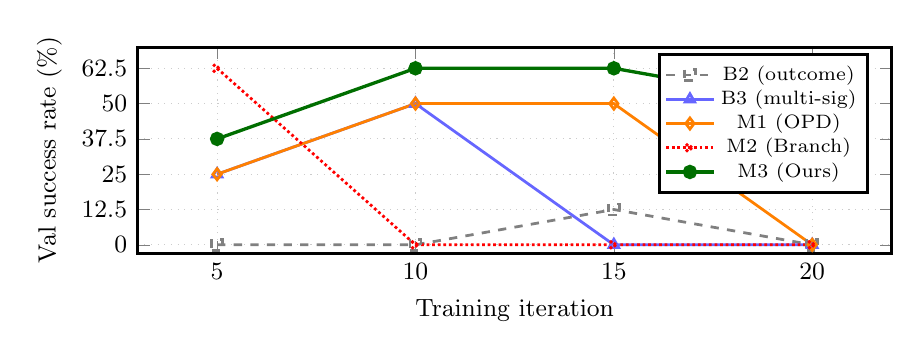
\begin{tikzpicture}
\begin{axis}[
  width=0.92\columnwidth, height=4.2cm,
  xlabel={Training iteration},
  ylabel={Val success rate (\%)},
  xtick={5,10,15,20},
  ytick={0,12.5,25,37.5,50,62.5},
  yticklabels={0,12.5,25,37.5,50,62.5},
  ymin=-3, ymax=70,
  xmin=3, xmax=22,
  legend pos=north east,
  legend style={font=\scriptsize, inner sep=2pt, row sep=-2pt},
  tick label style={font=\small},
  label style={font=\small},
  grid=major, grid style={dotted,gray!40},
  line width=1pt,
]
\addplot[color=gray,  mark=square,  dashed] coordinates {(5,0)(10,0)(15,12.5)(20,0)};
\addplot[color=blue!60,  mark=triangle] coordinates {(5,25)(10,50)(15,0)(20,0)};
\addplot[color=orange, mark=diamond] coordinates {(5,25)(10,50)(15,50)(20,0)};
\addplot[color=red,   mark=x,       densely dotted] coordinates {(5,62.5)(10,0)(15,0)(20,0)};
\addplot[color=darkgreen, mark=*, very thick] coordinates {(5,37.5)(10,62.5)(15,62.5)(20,50)};
\legend{B2 (outcome), B3 (multi-sig), M1 (OPD), M2 (Branch), M3 (Ours)}
\end{axis}
\end{tikzpicture}
\caption{\textbf{Validation success rate across training.}
M3 (green) is the only method with non-zero success at step 20.
M2 peaks earliest but collapses catastrophically (reward hacking).
M1 sustains longer but still collapses. M3 uniquely recovers from partial hacking at step 15.}
\label{fig:training_curve}
\end{figure}

\subsection{Analysis}

\textbf{Only M3 survives to step 20.}
Every baseline hits 0\% by iteration 20 (Table~\ref{tab:main}; Figure~\ref{fig:training_curve}).
M3 still solves half the tasks at that point --- Reward@20 = 0.979, the only value
that has not climbed past the task-success ceiling. Cum.\% = 212.5, versus 75 for B3
and 125 for M1.

\textbf{Ablation: neither component alone suffices.}
M2 (Branch only) achieves the highest single-checkpoint peak (62.5\% at step 5) but
collapses by step 10 (Reward@10 = 1.284, worst hacking observed): without
OPD's per-step signal, the agent learns to trigger branches by repeatedly failing
validation, accumulating branch rewards without resolving tasks.
M1 (OPD only) is more stable --- sustaining 50\% through steps 10 and 15 --- but
shows early hacking signs at step 15 (Reward@15 = 1.085) and collapses to 0\% test
success at step 20 (Reward@20 = 1.135). With OPD cap $= 2$, step rewards alone max
at $+0.2$; the elevated training reward at convergence reflects exploitation of the
$+0.3$ partial terminal credit (validate passes but \texttt{done} not called) and
training-distribution overfitting, neither of which transfers to test tasks.

\textbf{M3: transient hacking with self-correction.}
M3 partially hacks at step 15 (Reward = 1.151; honest expected reward
${\leq}0.625{\times}1.2 + 0.375{\times}0.2 = 0.83$ at 62.5\% success,
since failed episodes may receive zero step reward; OPD ceiling = 1.2),
indicating exploitation coexisting with genuine task-solving.
Crucially, M3 \emph{recovers} to Reward = 0.979 at step 20 while sustaining 50\% success ---
a trajectory absent in all baselines (Table~\ref{tab:hacking}).
Repeated validation failures trigger Error-Branch observations that force recovery reasoning;
OPD's gradient sustains productive learning. Transient-then-recovery distinguishes M3 from
methods that hack terminally.


% ============================================================
\section{Related Work}
\label{sec:related}

\textbf{Group-based agentic RL.}
GiGPO~\cite{zeng2025gigpo} establishes step-level group baselines via ex-post
anchor-state matching. HGPO~\cite{feng2026hgpo} refines this with hierarchical
context-consistent groups without extra rollouts; SPEAR~\cite{spear2026} augments
exploration via self-imitation and entropy scheduling. Error-Branch is orthogonal
to both: it actively forks rollouts at compiler-error states, adding new trajectories
conditioned on semantic signals---a direction neither HGPO nor SPEAR addresses.
The closest structural precedent is VinePPO~\cite{kazemnejad2024vineppo}, which
re-simulates $K$ continuations from intermediate states for Monte Carlo value estimation;
Error-Branch differs in both purpose (exploration concentration and anti-hacking rather
than credit assignment) and trigger (semantic compiler errors rather than content-agnostic
state sampling).

\textbf{RL from compiler feedback.}
CodeRL~\cite{le2022coderl}, RLTF~\cite{liu2023rltf}, and StepCoder~\cite{dou2024stepcoder}
all use compiler feedback, but in \emph{single-turn} generation: one program goes in, one verdict comes out.
Our departure is multi-turn agents where the policy controls \emph{when} to invoke the compiler
and reward hacking is an active failure mode.
MATH-Shepherd~\cite{wang2024mathshepherd} trains a learned PRM --- we use the compiler
directly (zero annotation cost, perfectly calibrated).
SWE-bench~\cite{jimenez2024swebench} uses test-suite pass rate; AGENTQ~\cite{putta2024agentq}
and RLAIF-Web~\cite{lai2024rlaifweb} use preference labels ---
our signal is deterministic and annotation-free.

% ============================================================
\section{Conclusion}
\label{sec:conclusion}

Compiler-as-Reward treats the compiler as what it actually is: a zero-cost oracle
that returns structured, content-specific error messages.
Compiler-OPD turns those into per-step training signal; Error-Branch uses
validation failures as branch points to concentrate exploration where the policy
is most uncertain. Together (M3), they hold 50\% task success through to the final
checkpoint --- Cum.\% = 212.5 --- while every baseline has collapsed.
M3 is still below Claude Sonnet 4 (81\% on this benchmark, direct API evaluation,
no RL training; cited as a practical ceiling), but it is the first RL-trained 4B model
with non-zero convergence performance on this evaluation.
The same logic applies wherever you have a validation API; we have not tested other domains yet.

\textbf{Human-centered implications.}
The compiler-driven recovery loop trained in M3 ---
validate error $\to$ branch $\to$ read schema $\to$ fix field $\to$ validate pass ---
mirrors the IDE debug cycle developers run intuitively.
Two things worth testing:
(1) \emph{Resume-after-interrupt}: Error-Branch's content-conditioned recovery should
transfer when a human pauses and redirects mid-task, since the recovery signal is
error content, not task identity.
(2) \emph{Interpretable traces}: compiler-derived observations give human collaborators
a readable failure log, unlike binary-reward agents with opaque rollouts.
A pair-programming study is the natural follow-up (see Appendix~\ref{app:trajectory}
for a representative M3 trajectory).

\textbf{Limitations.}
22 tasks, one theme, one seed. The trends look real but error bars matter;
multi-seed runs are the obvious next step.

% ============================================================
\bibliographystyle{plain}
\begin{thebibliography}{99}

\bibitem{le2022coderl}
Hung Le, Yue Wang, Akhilesh Deepak Gotmare, Silvio Savarese, and Steven C.H.\ Hoi.
\newblock CodeRL: Mastering Code Generation through Pretrained Models and Deep
  Reinforcement Learning.
\newblock In \emph{NeurIPS}, 2022.

\bibitem{liu2023rltf}
Jiate Liu, Yiqin Zhu, Kaiwen Xiao, Qiang Fu, Xiao Han, Wei Yang, and Deheng Ye.
\newblock RLTF: Reinforcement Learning from Unit Test Feedback.
\newblock \emph{arXiv:2307.04349}, 2023.

\bibitem{dou2024stepcoder}
Shihan Dou, Yan Liu, Haoxiang Jia, Limao Xiong, Enyu Zhou, Wei Shen,
  Junjie Shan, Caishuang Huang, Xiao Wang, Xiaoran Fan, Zhiheng Xi,
  Yuhao Zhou, Tao Ji, Rui Zheng, Qi Zhang, and Tao Gui.
\newblock StepCoder: Improve Code Generation with Reinforcement Learning from
  Compiler Feedback.
\newblock In \emph{ACL}, 2024.

\bibitem{zeng2025gigpo}
Xiangxiang Zeng, Feng Lang, et al.
\newblock GiGPO: Group-in-Group Policy Optimization for LLM Agent Training.
\newblock In \emph{NeurIPS}, 2025.
\newblock \url{https://github.com/langfengQ/verl-agent}

\bibitem{shao2024grpo}
Zhihong Shao, Peiyi Wang, Qihao Zhu, Runxin Xu, Junxiao Song,
  Mingchuan Zhang, Y.K.\ Li, Y.\ Wu, and Daya Guo.
\newblock DeepSeekMath: Pushing the Limits of Mathematical Reasoning in Open
  Language Models.
\newblock \emph{arXiv:2402.03300}, 2024.

\bibitem{jimenez2024swebench}
Carlos E.\ Jimenez, John Yang, Alexander Wettig, Shunyu Yao, Kexin Pei,
  Ofir Press, and Karthik Narasimhan.
\newblock SWE-bench: Can Language Models Resolve Real-World GitHub Issues?
\newblock In \emph{ICLR}, 2024.

\bibitem{qwen35}
Qwen Team.
\newblock Qwen3.5 Technical Report.
\newblock \emph{arXiv:2505.09388}, 2025.

\bibitem{wang2024mathshepherd}
Peiyi Wang, Lei Li, Zhihong Shao, R.X.\ Runxin Xu, Damai Dai,
  Yifei Li, Deli Chen, Yu Wu, and Zhifang Sui.
\newblock Math-Shepherd: Verify and Reinforce LLMs Step-by-step without Human
  Annotations.
\newblock In \emph{ACL}, 2024.

\bibitem{putta2024agentq}
Sneha Putta, Edmund Mills, Naman Garg, Suraj Wadhwa, Shyam Sundhar Ramesh,
  Eric Kolve, Roozbeh Mottaghi, Aniruddha Kembhavi, Luca Weihs, and
  Ranjay Krishna.
\newblock Agent Q: Advanced Reasoning and Learning for Autonomous AI Agents.
\newblock \emph{arXiv:2408.07199}, 2024.

\bibitem{lai2024rlaifweb}
Junhao Lai, Tianhao Yu, Kang Xu, and Weiran Huang.
\newblock RLAIF-Web: Alignment for Web Agents via Preference-based Reinforcement
  Learning.
\newblock \emph{arXiv:2402.10710}, 2024.

\bibitem{kazemnejad2024vineppo}
Amirhossein Kazemnejad, Milad Aghajohari, Eva Portelance, Alessandro Sordoni,
  Siva Reddy, Aaron Courville, and Nicolas Le Roux.
\newblock VinePPO: Unlocking RL Potential For LLM Reasoning Through Refined
  Credit Assignment.
\newblock \emph{arXiv:2410.01679}, 2024.

\bibitem{feng2026hgpo}
Shuo He, Lang Feng, Qi Wei, Xin Cheng, Lei Feng, and Bo An.
\newblock Hierarchy-of-Groups Policy Optimization for Long-Horizon Agentic Tasks.
\newblock In \emph{ICLR}, 2026.
\newblock \emph{arXiv:2602.22817}.

\bibitem{spear2026}
Yulei Qin, Xiaoyu Tan, Zhengbao He, Gang Li, Haojia Lin, Zongyi Li,
  Zihan Xu, Yuchen Shi, Siqi Cai, Renting Rui, Shaofei Cai, Yuzheng Cai,
  Xuan Zhang, Sheng Ye, Ke Li, and Xing Sun.
\newblock Learn the Ropes, Then Trust the Wins: Self-imitation with Progressive
  Exploration for Agentic Reinforcement Learning.
\newblock \emph{arXiv:2509.22601}, 2025.

\end{thebibliography}

% ============================================================
\appendix
\section{Representative M3 Recovery Trajectory}
\label{app:trajectory}

The following abridged trace shows M3 on an L2 task (\emph{``Add a testimonials section
with customer name and quote fields''}), illustrating the validate→branch→fix→pass loop.

\vspace{4pt}
\noindent\small
\begin{tabular}{@{}lp{0.78\columnwidth}@{}}
\toprule
\textbf{Step} & \textbf{Action / Observation (abridged)} \\
\midrule
1 & \texttt{read\_file(templates/index.json)} $\to$ current schema loaded \\
2 & \texttt{get\_section\_schema("testimonials")} $\to$ required fields: \texttt{customer\_name}, \texttt{quote} \\
3 & \texttt{write\_file} --- adds \texttt{"type":"testimonials","settings":\{...\}} \\
4 & \texttt{validate} $\to$ \textcolor{darkred}{\textbf{ERROR}}: \texttt{missing required field: quote} \\
  & \emph{[Error-Branch fires: k=4 continuations injected with error observation]} \\
5 & (k{=}4 branch; this continuation reached validate pass) \texttt{write\_file} --- adds \texttt{"quote":"Placeholder testimonial"} \\
6 & \texttt{validate} $\to$ \textbf{PASS} \\
7 & \texttt{done(status="success")} \\
\bottomrule
\end{tabular}
\vspace{4pt}

\noindent\normalsize
Step 4 triggers Error-Branch: the error message (\texttt{missing required field: quote}) is
injected as a structured observation into k{=}4 parallel continuations, each independently
rolled out and scored. The continuation shown (step 5) targets the specific missing field;
the other three either repeat the validation error or attempt unrelated edits.\footnote{%
Shopify's section schema validates field \emph{presence}, not content;
non-empty string values satisfy the constraint.}
OPD assigns $r_4{=}{+0.1}$ (first validate) and $r_6{=}{+0.1}$ (second validate),
plus $r_T{=}{+1.0}$ (resolved): total $R{=}1.2$.
B3 and M1 do not show this pattern: their validate calls keep firing
without responding to the error content.

\end{document}
